\section{Interactive Tool}

\subsection{Overview}

This interactive tool is an extension of the Urban Pulse interactive tool\cite{b1} and all the interaction strategies and widgets are of similar functionality. The interactive tool (Fig. 1) developed in this research combines the Map View and the Pulse Monitor components to allow users to explore the city's POIs by both POI type and the type of relationships they support. The tool is designed to enable users to gain a broad overview of the city's POIs, zoom and filter to seek finer details on individual entities and analyze the different properties of the pulses along with the activity across different temporal resolutions. The purpose of the tool is to support the exploration of pulses by both POI type and the type of relationships they support, in one or more cities and to enable the comparison of pulses across different scenarios within a city. The tool is intended for use by locals and tourists looking to find a venue to patronize under certain social contexts, as well as professionals aiming to understand how city layouts support different social relationships or where to put new businesses. The interactive tool (Fig. 3) is a powerful and innovative way to explore and analyze the relationship between POIs and social relationships in cities, providing users with a unique and informative experience.

\subsection{Features}
The interactive tool in Fig 1 shows the interface of the interactive tool. They can then select the relationship types (Fig. 4) they are interested in (e.g., "professional" or "romantic") using checkboxes, and optionally filter by POI type (e.g., "Restaurants" or "Arts \& Entertainment") using a dropdown menu. The tool offers several options to display the data: the raw number of relationship words, relationship word rate (number of words per 1000 reviews), or the percentage of relationship keywords in their reviews under that type. Users can limit the number of POIs to display on the map, where POIs with the highest relationship word rate (or raw count, or percent of words under the selected type) are shown.

Each point in the map is also color-coded based on the level of confidence in the presence of the selected relationship type in the reviews. POIs are symbolized by one of four different colors according to relationship type, and the color intensity increases with the level of confidence. Darker shades of a color indicate a higher confidence percentage of that relationship type in the reviews of that POI. The tool allows users to hover over POI points to see tooltips that include the name of the business and details about the relationship word occurrences in its reviews. Furthermore, users can limit the number of POIs to show on the map, wherein POIs with the highest relationship word rate (or raw count, or percent of words under the selected type) are drawn first. The tool also includes a sortable table of the POIs that are currently in view, which includes additional attributes such as the total number of reviews. Users can select a POI in the table and "jump" to it on the map, enabling exploration of different neighborhoods and serving as a reference through search capabilities. By providing zoomed-out snapshots of cities’ POIs, it also allows users to visually distinguish the prevalent relationships supported by various parts of a city and thus evaluate different parts of the city with relationships in mind. The tool also includes a sortable table of the POIs currently in view, which includes additional attributes such as the total number of reviews. Users can select a POI in the table and "jump" to it on the map. This feature enables the exploration of different neighborhoods and serves as a reference through search capabilities to look up specific POIs.

\begin{figure}
    \centering
    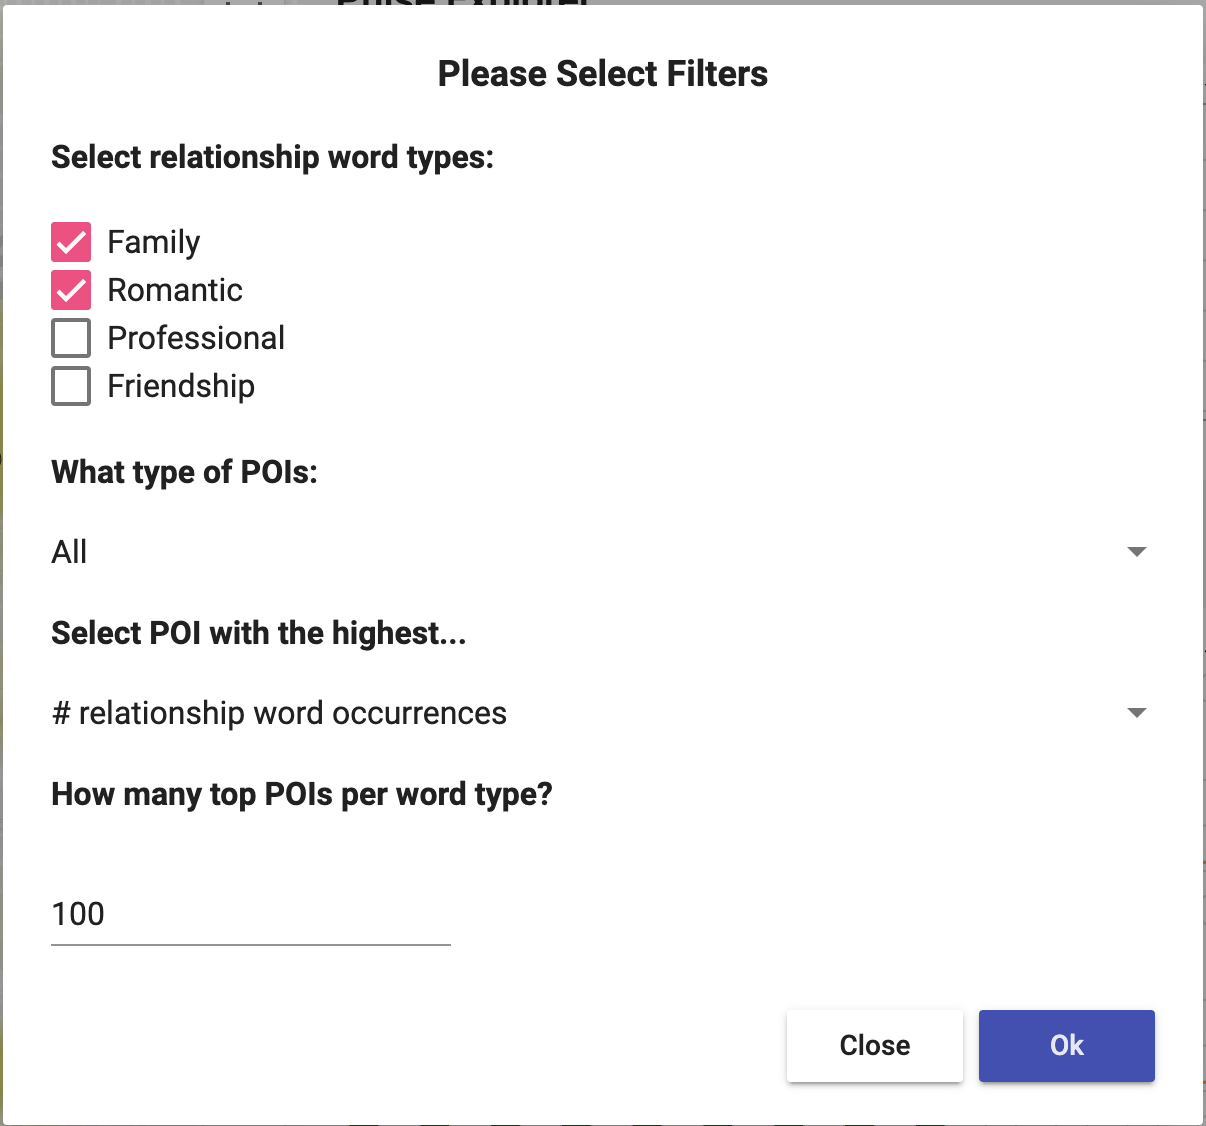
\includegraphics[width=\linewidth, height=6cm]{Filters.png}
    \caption{Options to interact with and filter on the tool}
    \label{fig:my_label}
\end{figure}

